\documentclass{bmvc2k}

%% Enter your paper number here for the review copy
% \bmvcreviewcopy{??}

% \usepackage[brazilian]{babel}
\usepackage[utf8]{inputenc}
\usepackage{placeins}

\title{Funções básicas do OpenCV}
 
% Enter the paper's authors in order
% \addauthor{Name}{email/homepage}{INSTITUTION_CODE}
\addauthor{Mateus de Moura Ramos Bittencourt}{bittenmat@gmail.com}{1}

% Enter the institutions
% \addinstitution{Name\\Address}
\addinstitution{
  Departamento de Ci\^encia da Comptuta\c{c}\~ao\\
  Universidade de Bras\'{\i}lia\\
  Campus Darcy Ribeiro, Asa Norte\\
  Bras\'{\i}lia-DF, CEP 70910-900, Brazil,  
}

\runninghead{Bittencourt, Mateus}{Computer Vision Assignment -- \today}

% Any macro definitions you would like to include
% These are not defined in the style file, because they don't begin
% with \bmva, so they might conflict with the user's own macros.
% The \bmvaOneDot macro adds a full stop unless there is one in the
% text already.
\def\eg{\emph{e.g}\bmvaOneDot}
\def\Eg{\emph{E.g}\bmvaOneDot}
\def\etal{\emph{et al}\bmvaOneDot}


%-------------------------------------------------------------------------
% Document starts here
\begin{document}

\maketitle

\begin{abstract}
This document demonstrates some of the simplest functions to image processing and computer vision on OpenCV. It contains examples of its usage and the result as well. The main library used on these programs was OpenCV, followed by numpy. Every non-intuitive function or logic implementation will be explained here.
\end{abstract}

%-------------------------------------------------------------------------
\section{Introdução}
\label{sec:intro}
Visão computacional e processamento de imagens são duas áreas muito próximas, ambas contendo várias características atrelaçadas. Neste trabalho, foi utilizado técnicas de processamento de imagem de forma a integrar a imagem ou o video com o mouse. Para isso, utilizou-se duas bibliotecas principais, OpenCV e Numpy. 

\subsection{OpenCV}
OpenCV, ou Open Computer Vision, é uma biblioteca de visão computacional fundada pela Intel em 2000, que passou por várias empresas, até retornar a intel e tornar-se open source, que permite a qualquer um editar. Atualmente, na versão 4.1, essa biblioteca pode ser usada para várias linguagens e sistemas operacionais. Pode-se dizer que grande parte do avanço na área de visão computacional deve-se à popularização dessa biblioteca.

 \cite{opencv_library}


\subsection{Numpy}
O trabalho aqui feito, foi realizado em python e uma de suas bibliotecas mais conhecidas, a numpy. Numpy é uma biblioteca de uso científico, que contém funções pre implementadas para facilitar o uso de matriz, vetor, e algebra como um todo. Criada por Travis Oliphant em 2005, foi amplamente usada ao longo dos anos e atualmente também é uma biblioteca aberta a todos.

\section{Problema Proposto}

\subsection{Integração mouse-imagem}
O primeiro problema proposto consiste em abrir uma imagem e ao clicar em algum ponto da imagem, retornar os valores de RGB se esta for colorida, ou intesidade de cinza se esta for em grayscale, assim como as coordenadas do ponto.

 \cite{splitshapemerge}
 \cite{MouseCallback}

\subsection{Destacar uma relação entre pixels em uma imagem}
Nesta seção, após selecionar um pixel na imagem, pixels com uma distancia euclidiana de cor menor que 13 deviam ser destacados, caso a imagem seja colorida, e uma diferença de intensidade menor que 13 no caso grayscale.

\cite{colorspaces}

\subsection{Destacar uma relação entre pixels em um vídeo}
O desafio dessa parte se mantém, porém agora com um vídeo. Isso é, ao clicar o valor do pixel é armazenado e comparado à todos os pixels do frame. Ao mudar de frame, o pixel clicado se mantem e compara-se aos novos pixels da imagem.

\subsection{Destacar uma relação entre pixels na webcam}
O problema final é repetir o problema de achar a relação entre pixels, porém agora em um vídeo gerado na webcam em tempo real.

\section{Metodologia}
 

Para destacar uma área considerada "próxima" ao pixel clicado em uma imagem, uma nova imagem era criada em uma nova janela, contendo os mesmo pixels da imagem original, porém com os pixels analisados como "próximos" pintados de uma cor só.

Para obter uma relação de pixels como foi feito no trabalho, foi necessário fazer a distância euclidiana para imagens coloridas. Para isso, clicou-se num pixel da imagem e se obteve os valores de azul ($B_1$), verde ($G_1$) e vermelho ($R_2$). A comparação com outro pixel qualquer ($B_2$, $G_2$, $R_2$) se da pela fórmula:

\begin{equation}
    Dist = \sqrt{((B_1 - B_2)^2 + (G_1 - G_2)^2 + (R_1 - R_2)^2)}
\end{equation}

Caso a imagem esteja em grayscale, basta subtrair o valor do pixel clicado com o pixel analisado. Caso seja menor que 13 ele deveria receber o destaque.

Vale ressaltar que o processamento em python de uma matriz, passando pixel a pixel resultaria em um atraso muito grande, pois seria um loop dentro de um loop, ordem ($n^2$), portanto para reduzir esse tempo de processamento uma lógica nova foi implementada. A partir do pixel clicado uma imagem nova é gerada contendo somente esse pixel, e te tamanho igual ao tamanho da imagem original. A partir disso, subtrai-se essa imagem da original e guarda o resultado numa imagem de distâncias. A partir dela, operações lógicas são aplicadas de forma a pintar de vermelho todos os pixels que possuem distância menor que 13. Dessa forma, não é necessário nenhum loop para analisar todos os pixels.

\cite{threshold}
\cite{noloop}
\cite{MatForImage}

\subsection{Vídeos e webcam}
Como dito anteriormente, para analisar um vídeo basta analisar várias imagens em sequência. Para isso criou-se um loop de visualização de frames com a condição de parada de que o próximo frame seja igual ao número total de frames do vídeo. Caso isso ocorra o vídeo acaba e a janela se encerra.
A análise da webcam se dá da mesma forma, analisando frame a frame, porém não há contagem de frames, portanto para se encerrar o usuário deve clicar a tecla esc ou cancelar o código através do terminal.

\section{Resultados}
Aqui estão alguns dos resultados obtidos com os problemas propostos:

\begin{figure}[!h]
    \centering
    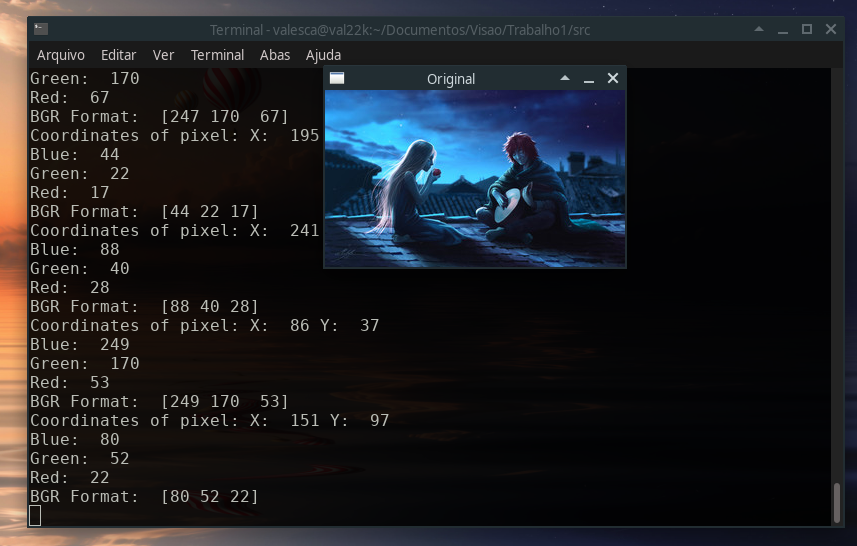
\includegraphics[width=0.9\textwidth]{Figs/trab1.png}
    \caption{Resultado do primeiro problema proposto}
    \label{fig:trab1}
\end{figure}

\begin{figure}[!h]
    \centering
    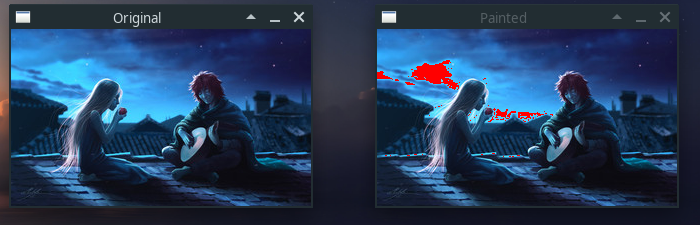
\includegraphics[width=0.9\textwidth]{Figs/trab2.png}
    \caption{Resultado do segundo problema proposto}
    \label{fig:trab2}
\end{figure}

\begin{figure}[!h]
    \centering
    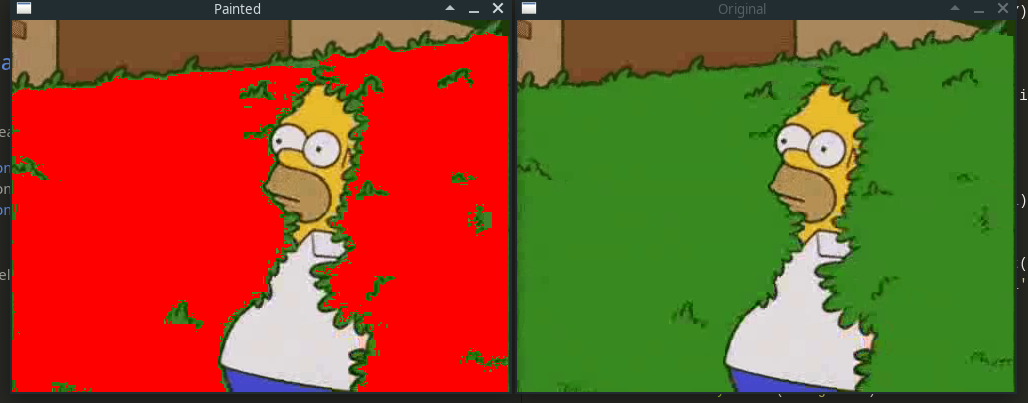
\includegraphics[width=0.9\textwidth]{Figs/trab3.png}
    \caption{Resultado do terceiro problema proposto}
    \label{fig:trab3}
\end{figure}
 \FloatBarrier

\begin{figure}[!h]
    \centering
    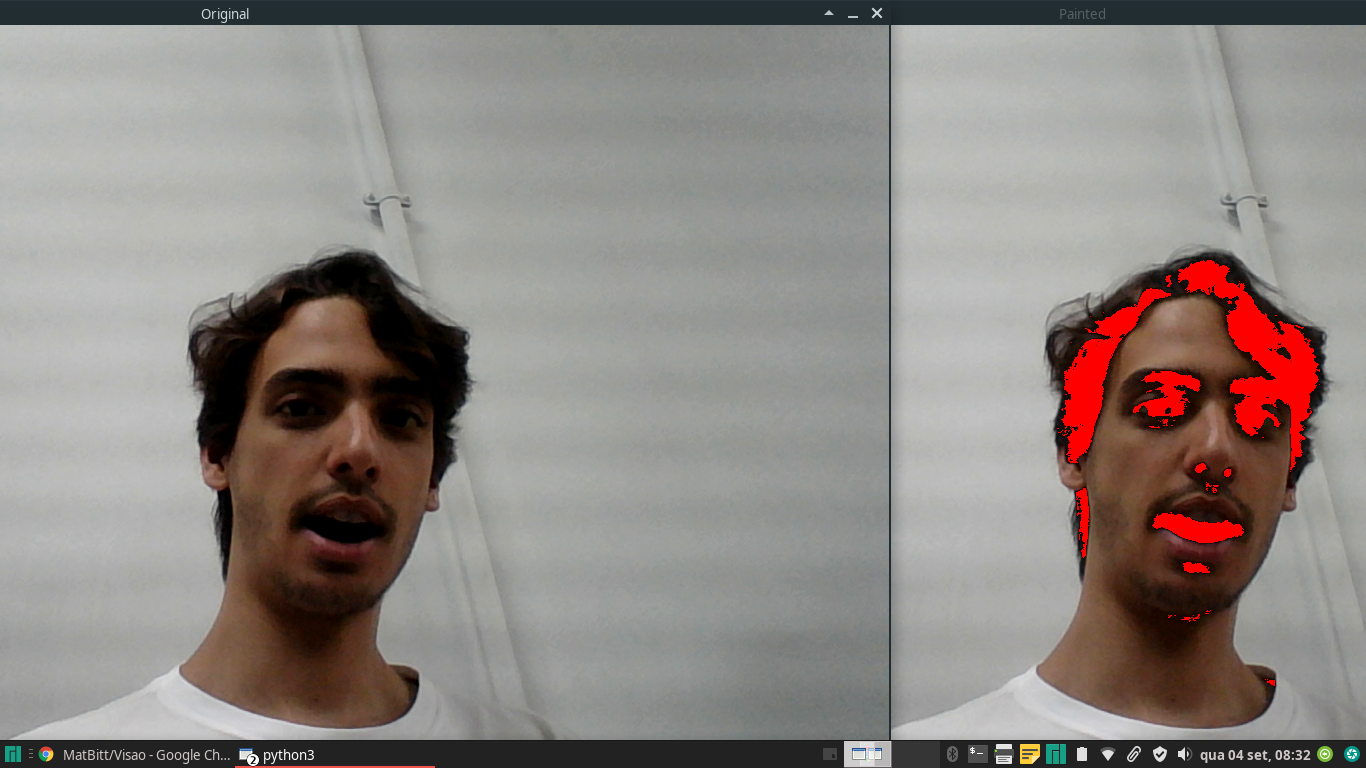
\includegraphics[width=0.9\textwidth]{Figs/trab4.png}
    \caption{Resultado do quarto problema proposto}
    \label{fig:trab4}
\end{figure}
 \FloatBarrier


\section{Discussão e Conclusão}
    Os resultados obtidos aqui foram satisfatórios e consistentes. Percebe-se nas imagens presentes na aba de resultados que os problemas propostos foram solucionados. 
    
    Python possui uma vasta gama de funções pré implementadas que facilitam o manuseio de matrizes e vetores, com a biblioteca numpy, mas isso acarreta numa demora maior para o processamento das mesmas. Portanto loops para essa linguagem são altamente não recomendáveis. Nesse trabalho, esse problema foi contornado com sucesso, através de operações lógicas e transposição de matrizes.
    
    Por fim, não houve nenhum atraso aparente na webcam, apresentando resultados muito bons também.

\bibliography{refs}
\end{document}
